
\documentclass[12pt, a4paper]{report}
\usepackage{graphicx}
\usepackage{amsmath}
\usepackage{float}


\title{\textbf{EE2703 : Applied Programming Lab \\ Assignment 5 \\Laplace Equation}} % Title

\author{Puneet Sangal\\ EE19b133} % Author name

\date{March 26, 2021} % Date for the report

\begin{document}		
		
\maketitle % Insert the title, author and date
\section*{1. Abstract}
We wish to solve for the currents in a resistor. The currents depend on the shape of the resistor and we also want to know which part of the resistor is likely to get hottest.

\section*{2. Introduction}
A wire is soldered to the middle of a copper plate and its voltage is held at 1 Volt. One side of the plate is
grounded, while the remaining are floating. The plate is 1 cm by 1 cm in size.
\\
We use Folloowing equations:
\begin{equation}
    \nabla \cdot \vec{j} = - \frac{\partial\rho}{\partial t}
\end{equation}
\begin{equation}
     \vec{j} = \sigma\vec{E}
\end{equation}
These equation give for dc current as folllows:
\begin{equation}
   \nabla^2 \phi =  0
\end{equation}

\section*{3. Assignment Problems}
 
 \subsection*{3.1 Defining the Parameters}
  We can initialize the parameters as passing the system arguments or we have default parameters as defined below:
  
  \begin{verbatim}
   if(len(sys.argv)==5):
     Nx=int(sys.argv[1])
     Ny=int(sys.argv[2])
     radius=int(sys.argv[3])
     Niter=int(sys.argv[4])
     print("Using user provided params")
   else:
     Nx=25                                            
     Ny=25                                           
     radius=8                                         
     Niter=1500                                      
  \end{verbatim}
  
 \subsection*{3.2 Initilazing and Plotting Potential}
  We have consider a radius of circle for which the potential remain constant, which gives the following contour plot as shown in figure:
  \begin{figure}[H]
	\centering
	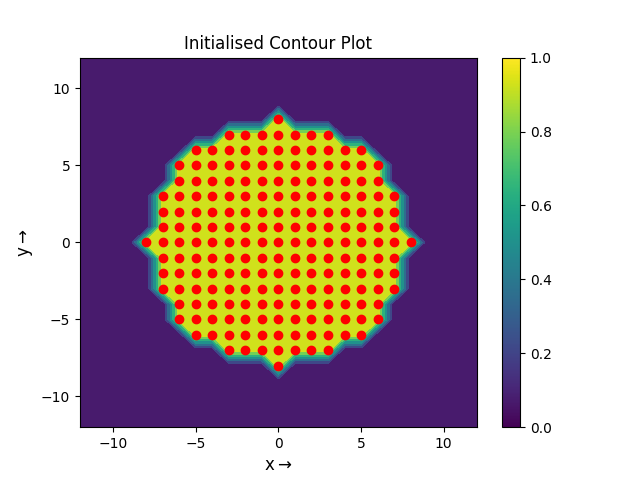
\includegraphics[scale=0.8]{Figure_1.png} 
	\caption{Part2: Initial Potential Configuration}
	\label{fig:1}
  \end{figure}
  
 \subsection*{3.3 Performing Iterations}
 We have to change the Potential after every Iteration which depends on the neighbouring average of old potential and boundary conditions as shown in following snippet:
 \begin{verbatim}
    def err_each_iteration(Niter,phi,err,ii):
    for k in range(Niter):
        phiold = phi.copy()
        phi = upd_phi(phi,phiold)
        phi = bound(phi,ii)
        err[k] = np.max(np.abs(phi-phiold)                                   
  \end{verbatim}
  
  \subsubsection*{3.3.1 Updating Potential}
  We have Upload the Potential by taking the average of the neighbouring old potential as follows:
  \begin{verbatim}
  def upd_phi(phi,phiold):
    phi[1:-1,1:-1]=0.25*(phiold[1:-1,0:-2]+
    phiold[1:-1,2:]+ phiold[0:-2,1:-1] + phiold[2:,1:-1])
    return phi
  \end{verbatim}
  
  \subsubsection*{3.3.2 Boundary Conditions}
  The following conditions as used for boundary:
  \begin{verbatim}
  def bound(phi,ii):
    phi[:,0]=phi[:,1]                    
    phi[:,Nx-1]=phi[:,Nx-2]             
    phi[0,:]=phi[1,:]                
    phi[Ny-1,:]=0
    phi[ii]=1.0
    return phi
  \end{verbatim}
 
 \subsection*{3.4 Plotting the Error}
  The found out the error in each term and represent on different Scales and found out that error is falling at a very slow rate, which is the major drawback of Laplace equation.The graphs are as follows:
  \begin{figure}[H]
	\centering
	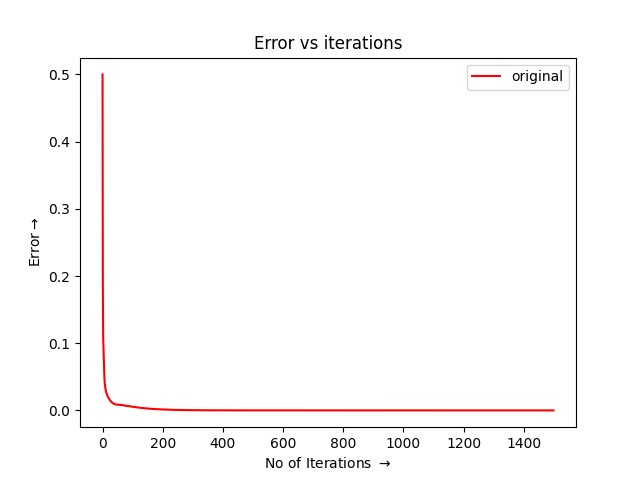
\includegraphics[scale=0.8]{Figure_2.png} 
	\caption{Part4: Error vs Iteration }
	\label{fig:2}
  \end{figure}
  \begin{figure}[H]
	\centering
	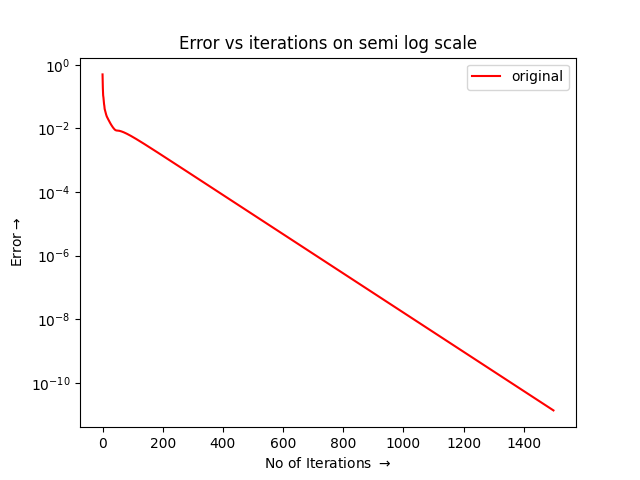
\includegraphics[scale=0.8]{Figure_3.png} 
	\caption{Part4: Error vs iteration on semi-log scale}
	\label{fig:3}
  \end{figure}
  \begin{figure}[H]
	\centering
	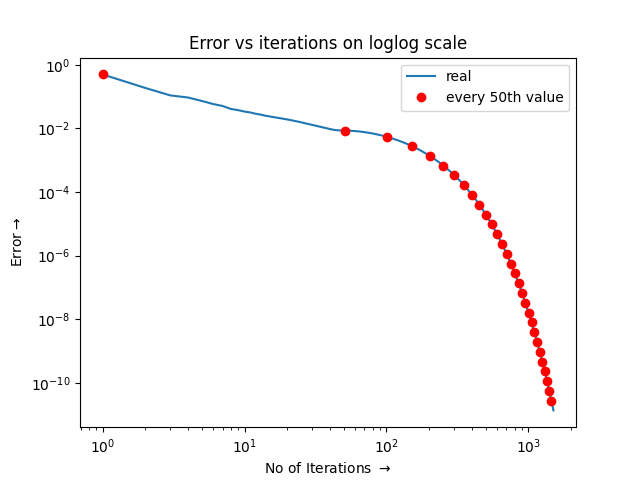
\includegraphics[scale=0.8]{Figure_4.png} 
	\caption{Part4: Error vs iteration on log-log scale}
	\label{fig:4}
  \end{figure}
  
 \subsection*{3.5 Fitting The Error}
  As we have seen the error is falling exponentially for higher iteration. So, we try to fit error for two fits. Fit-1, we have take all iterations and Fit-2, We have take iterations greater than 500. We use \texttt{scipy.linalg.lstsq()} to get fit the error.
  The graph are as follows:
  \begin{figure}[H]
	\centering
	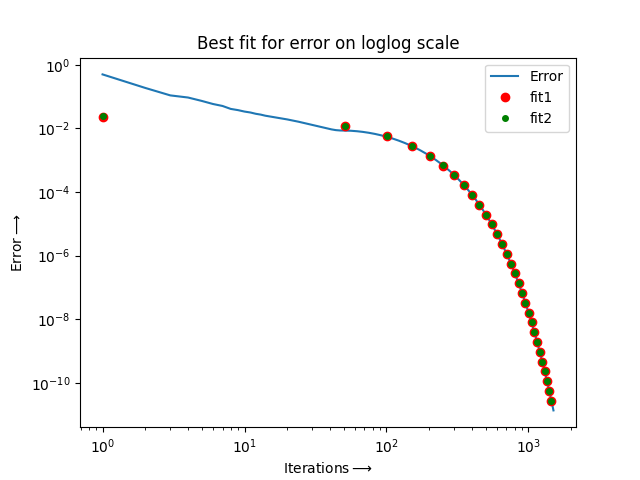
\includegraphics[scale=0.8]{Figure_6.png}
	\caption{Part5: Best fit of error on semi-log scale}
	\label{fig:6}
  \end{figure}
  \begin{figure}[H]
	\centering
	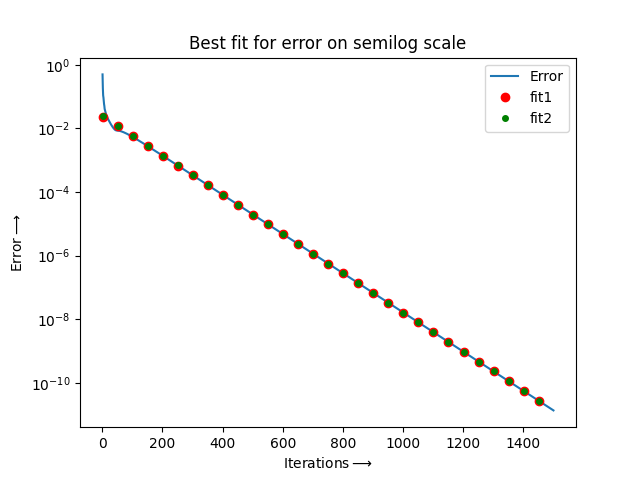
\includegraphics[scale=0.8]{Figure_5.png}
	\caption{Part5: Best fit of error on log-log scale}
	\label{fig:5}
  \end{figure}
  
 \subsection*{3.6 Potting cumulative Error}
  For each iteration, we try to find the cumulative error.This show how slowly the error is falling per iteration which is the worst assumption in Laplace equation, which can be seen as below:
   \begin{figure}[H]
	\centering
	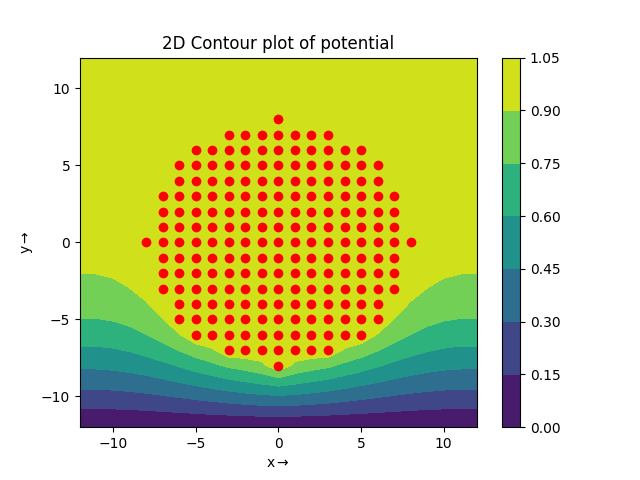
\includegraphics[scale=0.8]{Figure_7.png}
	\caption{Part6: Cumulative error vs number of iterations}
	\label{fig:7}
  \end{figure}
 
 \subsection*{3.7 Plotting Potential after Iterations}
  We plot the contour and 3-D plot of the Potential after last iterations as given by the user input. The graphs are as follows:
  
  \begin{figure}[H]
	\centering
	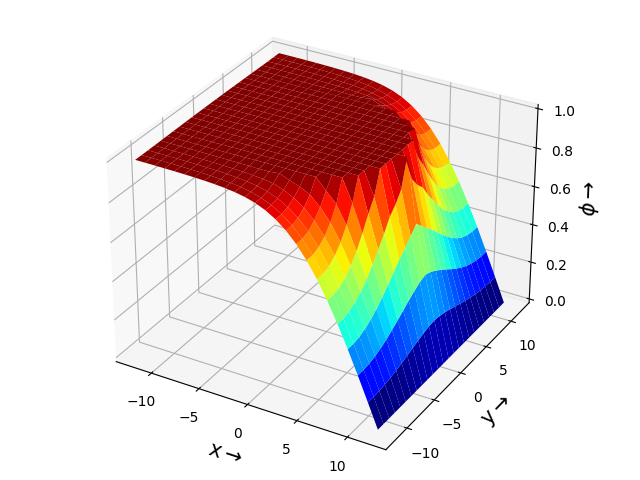
\includegraphics[scale=0.8]{Figure_8.png} 
	\caption{Part7: Contour Plot of Potential}
	\label{fig:8}
  \end{figure}
  
  \begin{figure}[H]
	\centering
	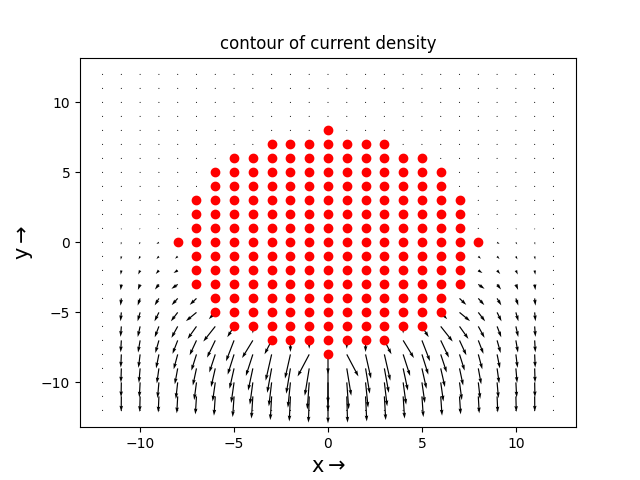
\includegraphics[scale=0.8]{Figure_9.png} 
	\caption{Part7: 3-D plot of Potential}
	\label{fig:10}
  \end{figure}
 
 \subsection*{3.8 Finding and Plotting the current density}
  We found out the current density by using following formula as shown in this snippet.
  \begin{verbatim}
      Jx,Jy = (1/2*(phi[1:-1,0:-2]-phi[1:-1,2:]),
               1/2*(phi[:-2,1:-1]-phi[2:,1:-1]))
  \end{verbatim}
  To Plot the current we used the \texttt{quiver} function , which show the following plot:
  \begin{figure}[H]
	\centering
	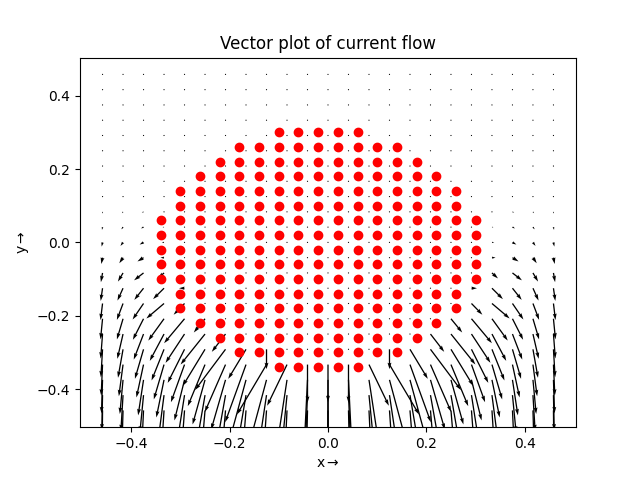
\includegraphics[scale=0.8]{Figure_11.png} 
	\caption{Part7: Current Density}
	\label{fig:0}
  \end{figure}
  
  From the plot, we have been able to see that current is flowing from below half plate and no current, is flowing through the upper half- plate. As lower surface is grounded, which shows that the most charge will from it.
  
 \subsection*{3.8 Finding and Plotting the Temperature in resistor}
 We have used the same concept as we used to find potential after iteration, to find the temperature , but here we have two extra terms from the current densiity and gives the following graph as shown:
  \begin{figure}[H]
	\centering
	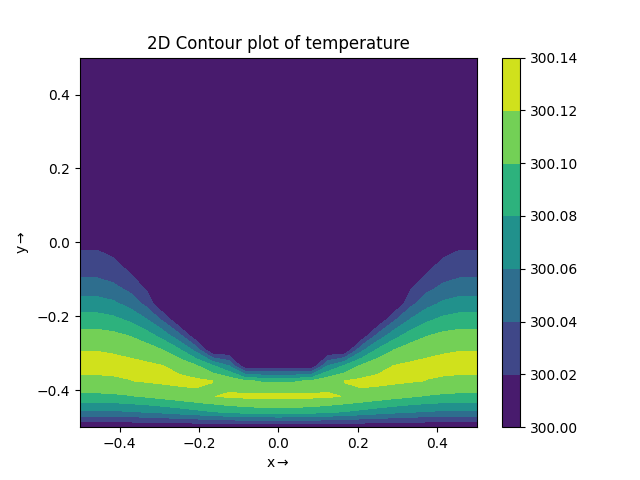
\includegraphics[scale=0.8]{Figure_12.png} 
	\caption{Part8: Dependence of Temperature}
	\label{fig:12}
  \end{figure}
  
  From graph, we can see that temperature will be maximum , where there is maximum flow of current, near the lower node.
  
  \section*{Conclusion}
  Using the Finite discrete Laplace equation, We found out the solution of the given system. Here, we saw that error is decaying at a very slow rate, which shows that choosing Laplace equation is inefficient. And from current density graph, current is flowing through the bottom half of the wire and is perpendicular to conductor as well as the temperature is maximum near lower part.

\end{document}



 
